%% two_stages.tex — Two-stage decomposition overview (compact, single-column)
%% Rendered via \resizebox{\linewidth}{!}{\input{...}} inside figure

\usetikzlibrary{positioning, arrows.meta, calc, fit, backgrounds, shapes.geometric}

%% ── Reuse the muted academic palette from v4_arch.tex ──
\providecommand{\definecolorIfNew}[2]{}
\definecolor{S1Blue}{RGB}{52,100,158}
\definecolor{S1BgCol}{RGB}{232,240,252}
\definecolor{S1Bdr}{RGB}{110,150,200}

\definecolor{S2Col}{RGB}{130,30,50}
\definecolor{S2Bg}{RGB}{250,232,236}
\definecolor{S2Bdr}{RGB}{175,60,80}

\definecolor{BranchACol}{RGB}{180,100,30}
\definecolor{BranchABg}{RGB}{253,245,228}
\definecolor{BranchABdr}{RGB}{200,140,60}

\definecolor{BranchBCol}{RGB}{38,120,90}
\definecolor{BranchBBg}{RGB}{228,248,238}
\definecolor{BranchBBdr}{RGB}{70,160,110}

\definecolor{IOCol}{RGB}{60,60,70}
\definecolor{IOBg}{RGB}{240,240,244}
\definecolor{ShapeCol}{RGB}{80,80,95}

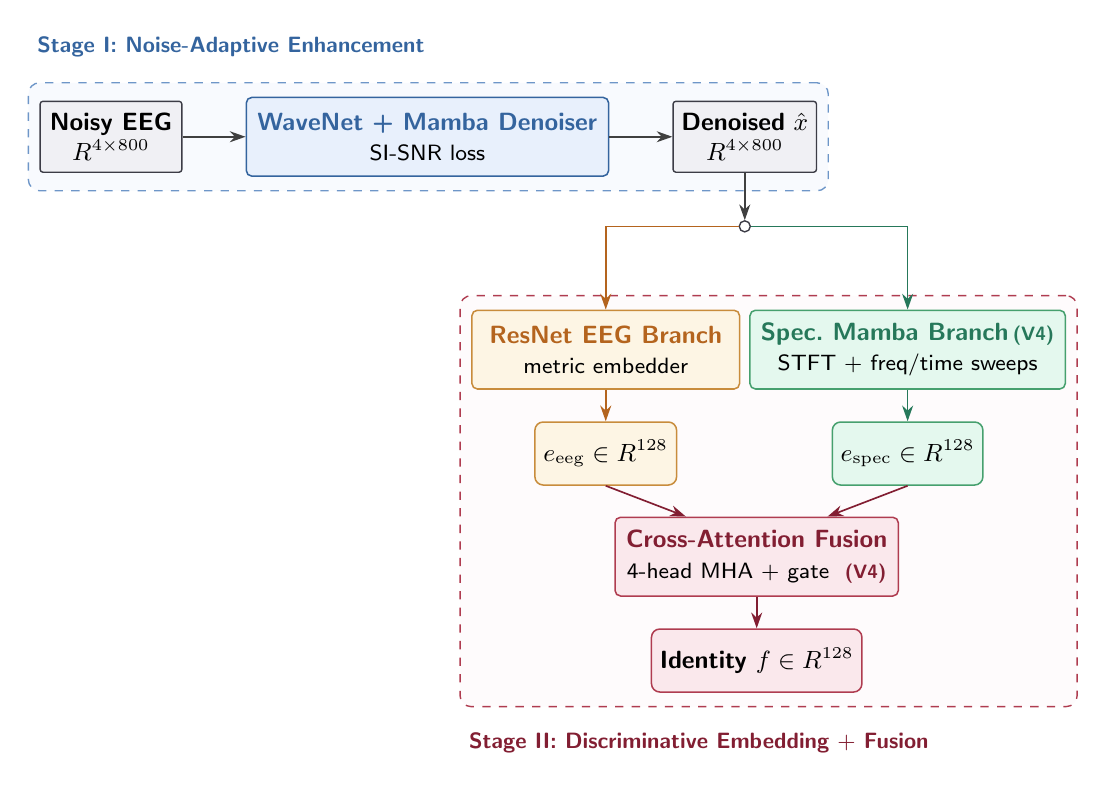
\begin{tikzpicture}[
    font=\small\sffamily,
    node distance=4mm and 6mm,
    >={Stealth[length=2.0mm, width=1.4mm]},
    every node/.style={align=center},
    blk/.style={
        draw, rounded corners=2pt,
        inner sep=4pt, minimum height=10mm,
        line width=0.55pt
    },
    ionode/.style={
        draw=IOCol, fill=IOBg, rounded corners=1pt,
        inner sep=3pt, minimum height=9mm, minimum width=18mm,
        line width=0.5pt, font=\small\sffamily
    },
    s1blk/.style={blk, draw=S1Blue, fill=S1BgCol, minimum width=34mm},
    ablk/.style={blk, draw=BranchABdr, fill=BranchABg, minimum width=34mm},
    bblk/.style={blk, draw=BranchBBdr, fill=BranchBBg, minimum width=34mm},
    fblk/.style={blk, draw=S2Bdr, fill=S2Bg, minimum width=30mm},
    embnode/.style={
        draw, rounded corners=3pt,
        inner sep=3pt, minimum height=8mm, minimum width=18mm,
        line width=0.55pt
    },
    splitnode/.style={
        circle, draw=IOCol, fill=white,
        inner sep=0pt, minimum size=4pt,
        line width=0.5pt
    },
    fl/.style={->, line width=0.55pt, draw=black!75},
    flA/.style={->, line width=0.55pt, draw=BranchACol},
    flB/.style={->, line width=0.55pt, draw=BranchBCol},
    flF/.style={->, line width=0.6pt, draw=S2Col},
    tlbl/.style={font=\scriptsize\itshape\sffamily, text=ShapeCol, inner sep=1pt},
    losslbl/.style={font=\scriptsize\sffamily, text=S1Blue, inner sep=1pt},
    stagelbl/.style={font=\footnotesize\bfseries\sffamily},
]

%% ── Stage I row ──
\node[ionode] (input) {%
    \textbf{Noisy EEG}\\
    $\mathbb{R}^{4\times 800}$%
};

\node[s1blk, right=8mm of input] (denoiser) {%
    \textcolor{S1Blue}{\textbf{WaveNet + Mamba Denoiser}}\\
    \footnotesize SI-SNR loss%
};

\node[ionode, right=8mm of denoiser] (denoised) {%
    \textbf{Denoised} $\hat{x}$\\
    $\mathbb{R}^{4\times 800}$%
};

%% ── Split into two branches ──
\node[splitnode, below=6mm of denoised] (split) {};

%% ── Stage II: Branch A (EEG/ResNet) ──
\node[ablk, below left=10mm and 0mm of split] (eegbr) {%
    \textcolor{BranchACol}{\textbf{ResNet EEG Branch}}\\
    \footnotesize metric embedder%
};

%% ── Stage II: Branch B (spectrogram/Mamba) — V4 addition ──
\node[bblk, below right=10mm and 0mm of split] (specbr) {%
    \textcolor{BranchBCol}{\textbf{Spec.\ Mamba Branch}\,\scriptsize\bfseries (V4)}\\
    \footnotesize STFT $+$ freq/time sweeps%
};

%% ── Branch embeddings ──
\node[embnode, draw=BranchABdr, fill=BranchABg, below=4mm of eegbr] (eegemb) {%
    $e_{\mathrm{eeg}}\in\mathbb{R}^{128}$%
};
\node[embnode, draw=BranchBBdr, fill=BranchBBg, below=4mm of specbr] (specemb) {%
    $e_{\mathrm{spec}}\in\mathbb{R}^{128}$%
};

%% ── Cross-attention fusion + identity vector ──
\node[fblk] at ($(eegemb.south)!0.5!(specemb.south) + (0,-9mm)$) (fusion) {%
    \textcolor{S2Col}{\textbf{Cross-Attention Fusion}}\\
    \footnotesize 4-head MHA $+$ gate~~\textcolor{S2Col}{\scriptsize\bfseries (V4)}%
};

\node[embnode, draw=S2Bdr, fill=S2Bg, below=4mm of fusion] (idvec) {%
    \textbf{Identity} $f\in\mathbb{R}^{128}$%
};

%% ── Arrows ──
\draw[fl] (input) -- (denoiser);
\draw[fl] (denoiser) -- (denoised);
\draw[fl] (denoised.south) -- (split);

\draw[flA] (split) -| (eegbr.north);
\draw[flB] (split) -| (specbr.north);

\draw[flA] (eegbr) -- (eegemb);
\draw[flB] (specbr) -- (specemb);

\draw[flF] (eegemb.south) -- ([xshift=-9mm]fusion.north);
\draw[flF] (specemb.south) -- ([xshift=9mm]fusion.north);

\draw[flF] (fusion) -- (idvec);

%% ── Background stage boxes ──
\begin{pgfonlayer}{background}
    \node[
        draw=S1Bdr, dashed, rounded corners=4pt,
        fill=S1BgCol, fill opacity=0.30,
        line width=0.5pt,
        fit=(input)(denoiser)(denoised),
        inner xsep=4pt, inner ysep=5pt
    ] (stage1box) {};

    \node[
        draw=S2Bdr, dashed, rounded corners=4pt,
        fill=S2Bg, fill opacity=0.18,
        line width=0.5pt,
        fit=(eegbr)(specbr)(eegemb)(specemb)(fusion)(idvec),
        inner xsep=4pt, inner ysep=5pt
    ] (stage2box) {};
\end{pgfonlayer}

%% ── Stage labels (top-left of each box) ──
\node[stagelbl, text=S1Blue,
      above=2mm of stage1box.north west, anchor=south west]
    {\textsc{Stage I}: Noise-Adaptive Enhancement};

\node[stagelbl, text=S2Col,
      below=2mm of stage2box.south west, anchor=north west]
    {\textsc{Stage II}: Discriminative Embedding $+$ Fusion};

\end{tikzpicture}
